\documentclass{article}

\usepackage{graphicx}
\usepackage{hyperref}


\graphicspath{ {Images/} }


\newcommand{\tab}[1]{\hspace{.1\textwidth}\rlap{#1}}

\begin{document}
	
\begin{titlepage}
	\newcommand{\HRule}{\rule{\linewidth}{0.5mm}} % Defines a new command for the horizontal lines, change thickness here

	\center % Center everything on the page
	 
	%----------------------------------------------------------------------------------------
	%	LOGO SECTIONS
	%----------------------------------------------------------------------------------------

	
\includegraphics[width=\textwidth]{./Images/front-page.jpg}

	%----------------------------------------------------------------------------------------
	%	TITLE SECTION
	%----------------------------------------------------------------------------------------

	\HRule \\[0.4cm]
	{ \huge \bfseries Architectural Requirements Specification and Design}\\[0.4cm] % Title of your document
	\HRule \\[0.5cm]
	{ \large \bfseries Eiffel Team }% Title of document
	{\large \bfseries - \today}\\
	\HRule \\[1.5cm]
	%----------------------------------------------------------------------------------------
	%	MEMBERS, TEAM NAME SECTION
	%----------------------------------------------------------------------------------------

	\begin{minipage}{0.5\textwidth}
	\emph{Members:}\\% add your name and student here
	Dilapisho Monkeli 15074260	
	
	Eksteen Ernst 28398603
	
	Haasbroek Henri-Dawid 15046657
	
	Mahoko  Dimpho 15175091
		
	van Schalkwyk John 14307317

	Veldsman Dian 12081095

	Mdluli Paul ----
	\end{minipage}
\end{titlepage}

\tableofcontents{}	

	\newpage
	\section{Introduction}
		\subsection{Purpose}
		The purpose of this document is to outline the design of the system to be developed. This document can be analysed from a more technical view point and is meant to be an technical outline for developers.  Similar to the requirements specification and the architectural specification, the design specification also forms part of a formal contract between developers and clients.
		\subsection{Document conventions}
			\begin{itemize}
				\item Documentation formulation:  LaTeX
				\item Architectural schemas: JGraph's \href{https://www.draw.io/}{Draw.io}
			\end{itemize}
		\subsection{References}
		\subsection{Related documents}
			\begin{itemize}
				\item \href{http://www.cs.up.ac.za/files/COS301/Download/1528/}{System Requirement Specification (SRS) for the NavUP System}
			\end{itemize}
	\section{System description}
	
	\section{Overall Architecture}
		\subsection{Architectural patterns}
		\subsection{Software system attributes}
		\subsection{Design constraints}
		\subsection{Technology and framework selection}
		
		
	\section{External Interface Requirements}
		\subsection{User Interfaces}
		\subsection{Hardware Interfaces}
		\subsection{Software Interfaces}
		\subsection{Communications Interfaces}
		
	\newpage	
	\section{Details of subsystem}
	\subsection{Subsystem Modules}
		\subsubsection{User Module}
		\subsubsection{Notifications Module}
			\paragraph	{Scope}\mbox{} \\
				\begin{figure}[h]
					\includegraphics[width=\textwidth]{./Images/Notification_Use_Case_v2.png} 
					\caption{Notification Module Use-Case Diagram}
				\end{figure}
			
				{The notification Module will provide end-users notifications with regards to the different aspects of the system, such as system updates or events taking place. Both subsystems as well as administrative users will use the notification system. The notification subsystem will send notifications either via email or SMS, depending on the end-user's noted preference.}		
		
			\newpage
			\paragraph	{Requirements, Interfaces and Constraints} \mbox{} \\
			{The system is required to be light weight and must be easily interfaced with to allow any subsystem that needs the ability to send a user a notification the ability to do so. It thus needs to be extremely moduler. \\ \\The Notification Module will need to interface with the user module, as it will need access to different users and their contact details as well as their preference methods of notification. The module will also need to provide a simple interface, as mentioned above, for simple messaging through the system. The Notification subsystem will also need to interface with an external browser or email client in order to send email to the UP email server so that those emails may in turn be forwarded to the end-user and/or an email to SMS gateway that will SMS the end-user.\\ \\The Notification Module will need to be able to built message all users, certain groups of users and specific users. The Notification Module will also need to be able to send time scheduled messages and as such be able to update said notifications or update them. Thus notifications must be retrievable.\\ \\Since the Notification Module does not host its own in application messaging system, the subsystem is constrained to interfacing with web based methods of communication through the use of email and gateways. This means that their is no way for the notification subsystem to know if the end-user has indeed reviewed their notification and thus can not create or send reminder notifications. There is also lot less control over the presentation and user experience of the notifications as they will have to conform to a standardised means of test presentation. However this means the system is easier to implement as a lot of leg work has already been done with regards to sending emails from software packages and frees developers up from creating a in application based notification system from scratch.}
		
			\newpage
			\paragraph	{Notification Module Structure} \mbox{} \\
			\begin{figure}[h]
				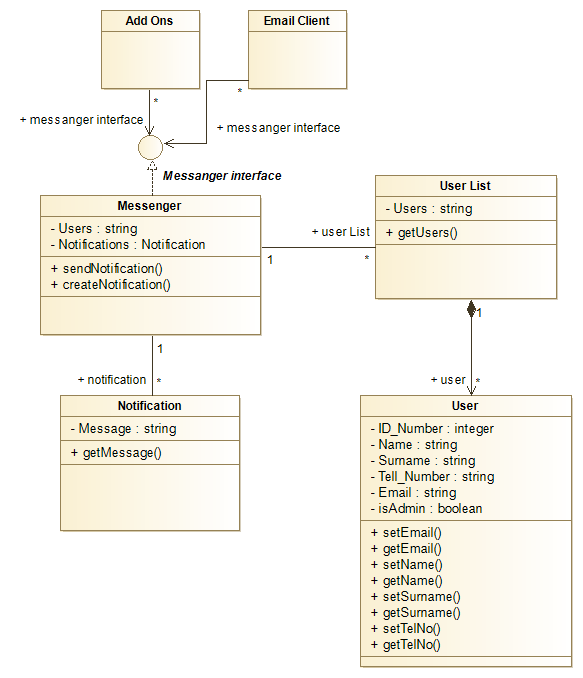
\includegraphics[width=\textwidth]{./Images/Notification_Class_Diagram.png} 
				\caption{Notification Module Class Diagram}
			\end{figure}
			
			{The Notification Module will provide a simple interface through which most communication and interaction with the subsystem will be done. This ensures a highly moduler design. This interface allows for easy message creation by creating notification with various overloaded functions. It also allows for notification retrieval, updating and deletion.\\ \\The NotificationsManager class implements the interface and provides the administrative functionality required to send notifications. It interfaces with the User Module to get users for their details by either getting users or lists of users, called user groups. Updates notifications and retrieves them from a stored list. It also ensures that notification are sent when they need to go out. Furthermore it tests the syntax structure of the message it is required to send before handing it off to the abstract factory class AbstractNotifcationFactory.\\ \\The AbstractNotificationFactory class is an interface that allows access to two concrete factories that implement a different concrete type of the Notification class. one being a email factory and the other being a SMS factory. Once these diffrent kinds of concreate Notification types have been created they are handed back to the NotificationsManger, which stores them for when they need to be sent.\\\\Using dependency injection, the NotificationsManager hands off the required notifications and users to the MessageSender class who interfaces with the required web technologies and handles the sending of notifications to each  or groups of end-user.}
		\subsubsection{Fitness Module}
		\subsubsection{Point Of Interest Module}
				\section{Point Of Interest Module}
		        \begin{figure}[h]
		            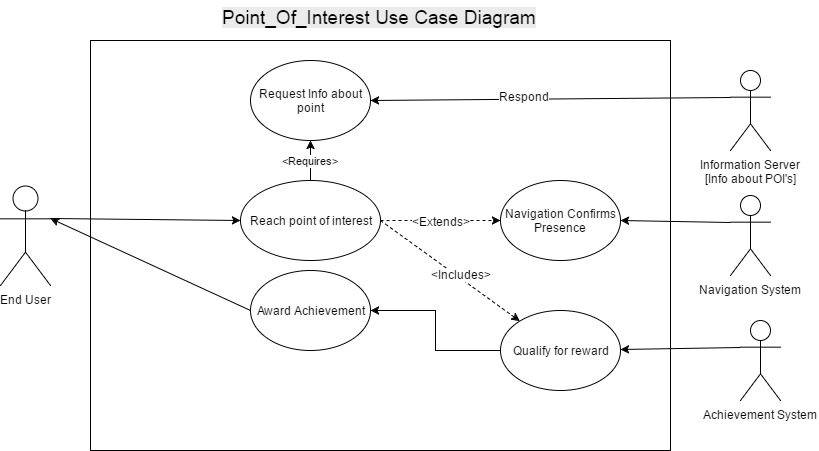
\includegraphics[width=\textwidth]{./Images/POI_Usecase.jpg} 
		            \caption{Point of interest module use case diagram}
		        \end{figure}

		        \begin{figure}[h]
		            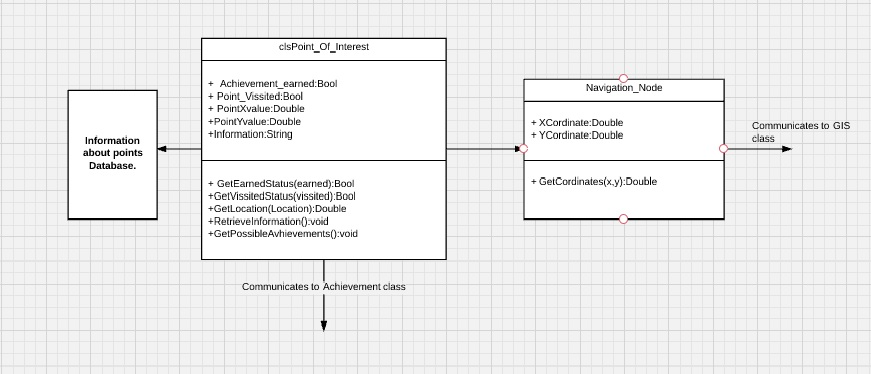
\includegraphics[width=\textwidth]{./Images/POI_Class.jpg} 
		            \caption{Point of interest module class diagram}
		        \end{figure}

{The point of interest module will be used to give an interface that will allow users to visit points of interest on campus and view information about the various points of interest. There are only 2 classes in this module, and those are the clsPoint_of_interest and the navigation_Node. The clsPoint_of_Interest will communicate with 3 sections, the database that contains all of the information about the particular point, and also with the Navigation node and lastly with the Achievements classes./// The Navigation_Node is used to retrieve the user's current location and match it with the point of interest's location to determine if the user is currently at the point. The Navigation_Node retrieves the user's location by communicating with the GIS and receiving the location. When the location is retrieved, it is requested by the clsPoint_of_Interest and then the information about the current point can be retrieved and displayed. The Point_Of_Interest needs to communicate with the achievement classes in order to determine if a user qualifies for an achievement or not}
		\newpage
		\subsection{Physical view}
	
			\begin{figure}[h]
				\includegraphics[width=\textwidth]{./Images/Deployment_Diagram.png} 
				\caption{Notification Module Class Diagram}
			\end{figure}
			
			{The NavUp system will primarily exist on its own network, but interfaces with the University of Pretoria's network at large to send and receive its data. Each subsystem will exist on its own server (virtual or physical) that will deal with incoming requests.\\\\This splitting of the system into several servers will ensure that no server is bogged down by a lack of resources or access time when dealing with the masses of concurrent end users. Thus the GIS server will be able to service users while the fitness server or navigation server periodically retrieve information from them on request, rather then having the server slow down under huge loads a end users try access GIS services and others their Fitness data, and others still update their user accounts.\\\\Subsystems that are closely linked will run on the same server and will only require each server accessing another server when certain information is required, else each server will be able to directly service the end-user without putting further strain on the other servers servicing other end-users.\\\\As the NavUp sub-network is connected to the UP network, administrative duties will be possible from an administrative terminal. The access to the UP network will also provide the NavUp network access to the UP Email Server to provide notification functionality which will then travel back through the network, out through the router and fire wall and to a gateway for emails and emails to SMS's and to the end-users device.\\\\The end users device will primarily have access to the NavUp system on campus through it's connection to WiFi Connection Points, that are found all over campus. These points will be utilised through the NavUp application and sent to the NavUp Server through the UP router, firewall and network to calculate GIS information. Similar methods and functions will be used to give the user real time access to the navigational subsystem and points of interest subsystem.////The NavUp User Server will maintain and deal with requests regarding the various systems requests for user data, and thus require its own server as multiple sub servers will require the updating of this server constantly. An achievements subsystem will also need to be implemented to maintain a higher degree of modularity when implementing a rewards program for end-users based on their fitness tracking as well as their exploration of campus.}
\end{document}

